\documentclass[tikz]{standalone}
\usepackage{pgfplots}
\pgfplotsset{compat=1.18} % Use a recent compat version
\begin{document}
	
	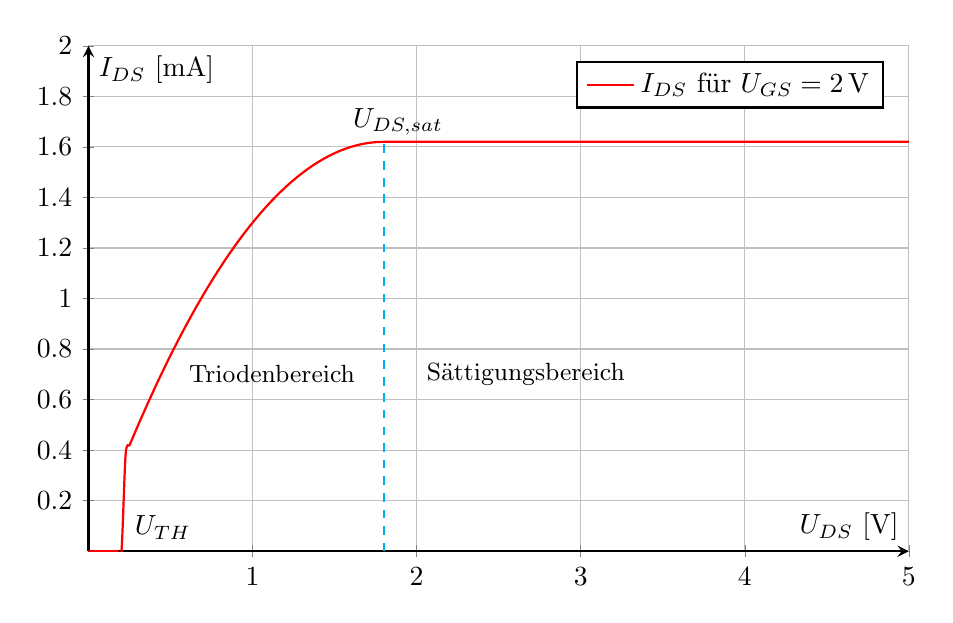
\begin{tikzpicture}
		\begin{axis}[
			width=12cm,
			height=8cm,
			axis lines=middle,
			xlabel={$U_{DS}$ [V]},
			ylabel={$I_{DS}$ [mA]},
			xmin=0, xmax=5,
			ymin=0, ymax=2,
			xtick={0,1,...,5},
			ytick={0,0.2,...,2.0},
			domain=0:5,
			samples=200,
			smooth,
			thick,
			grid=both,
			legend pos=north east,
			]
			
			% Durchgehende rote Linie für IDS
			\addplot[red, thick, domain=0:5] {
				x < 0.202 
				? 0
				: (x < 1.81 
				? 1*(2 - 0.2)*x - 0.5*x^2 
				: 1.62)
			};
			\addlegendentry{$I_{DS}$ für $U_{GS} = 2\,\mathrm{V}$}
			
			% Vertikale gestrichelte Linie bei U_DS = 1V
			\addplot[dashed, cyan, domain=0:1.62] coordinates {(1.8,0) (1.8,1.62)};
			\node[anchor=west] at (axis cs:1.55,1.7) {$U_{DS,sat}$};
			
			% Bereichsbeschriftungen
			% \node[anchor=west, font=\small] at (axis cs:0.05,0.05) {Sperrbereich};
			\node[anchor=west, font=\small] at (axis cs:0.55,0.7) {Triodenbereich};
			\node[anchor=west, font=\small] at (axis cs:2,0.7) {Sättigungsbereich};
			
			% Vertikale gestrichelte Linie bei U_TH = 0.2V
			
			% \addplot[solid, black, domain=0:0.15] coordinates {(0.2,-0.05) (0.2,0.05)};
			\node[anchor=north west, black] at (axis cs:0.22,0.18) {$U_{TH}$};
			
		\end{axis}
	\end{tikzpicture}
\end{document}
